\documentclass{beamer}
\mode<presentation>
{
\usepackage{external/dis-template}
}
\usepackage{listings}
\usepackage{textcomp}
\usepackage{svg}

\definecolor{comments}{HTML}{50c878}
\lstset{language=C++,
  basicstyle=\ttfamily,
  keywordstyle=\color{blue}\ttfamily,
  stringstyle=\color{red}\ttfamily,
  commentstyle=\color{comments}\ttfamily,
  breaklines=true
}

\graphicspath{{images/}} % TODO: eliminate this hack, necessary because scons builds at repository root

%---------------------------------------------------------------------
\titlepageinit{15}{Firmware Optimization and Engineering}{13 October 2016}
%---------------------------------------------------------------------
\begin{document}
%---------------------------------------------------------------------
\begin{frame}
\titlepage
\setcounter{tocdepth}{1}
\tableofcontents
\end{frame}

%---------------------------------------------------------------------
\section{Optimization} % [?? mins]
%---------------------------------------------------------------------
\begin{frame}
\centering \huge Optimization
\end{frame}


\subsection{Introduction}
%---------------------------------------------------------------------
\begin{frame}
\frametitle{Recap}
We brought up the basic hardware and firmware last time \\
\begin{itemize}
  \item Line camera
  \item Servo
  \item Line detection and controller loop
\end{itemize}
\hfill \break
But it's slow
\begin{itemize}
  \item For a fast car: will lose the line by the time steering updates
\end{itemize}
\hfill \break
\textbf{How do we optimize?}
\end{frame}


\begin{frame}
\frametitle{Optimizing}
How much should we optimize? \\
Or, what other limiting factors are there?

\visible<2-> {
\begin{itemize}
  \item Physical
  \visible<3-> {
    \begin{itemize}
      \item Camera exposure / integration time (50ms)
      \item Servo mechanical response (160ms / 60deg)
    \end{itemize}
  }
  \item Electrical
  \visible<3-> {
    \begin{itemize}
      \item Servo update rate (20ms)
    \end{itemize}
  }
\end{itemize}
}
\visible<4-> {
Just for fun, what are some ways around these?
}
\end{frame}


\begin{frame}
\frametitle{Measuring}
How can we measure the update rate? What are some trade-offs? \\

\visible<2-> {
\begin{itemize}
  \item \texttt{printf} and timers
  \item Logic analyzer / oscilloscope on external IO, like \texttt{Serial}
  \item Dedicated timing signals on external IO
\end{itemize}
}

What takes the most amount of time?
\end{frame}


\subsection{Optimizations}
%---------------------------------------------------------------------
\begin{frame}[fragile]
\frametitle{Overlapped / pipelined operations}
How can we optimize this?
\begin{lstlisting}[language=C++,basicstyle=\ttfamily\scriptsize]
camera.read_frame(data);  // discard to start integration
wait_ms(50);
camera.read_frame(data);  // actually read the frame
float steering = controller.update(line_detect(data)); // expensive
servo.write(steering);
float temperature = read_temperature();  // slow I2C I/O operations
\end{lstlisting}
\end{frame}


\begin{frame}[fragile]
\frametitle{Overlapped / pipelined operations}
How can we optimize this?
\begin{lstlisting}[language=C++,basicstyle=\ttfamily\scriptsize]
camera.read_frame(data);  // discard to start integration
wait_ms(50);
camera.read_frame(data);  // actually read the frame
float steering = controller.update(line_detect(data)); // expensive
servo.write(steering);
float temperature = read_temperature();  // slow I2C I/O operations
\end{lstlisting}
\hfill \break
Overlap temperature read and line detect with camera integration
\begin{lstlisting}[language=C++,basicstyle=\ttfamily\scriptsize]
timer.reset();
camera.read_frame(data);  // actually read the frame
float steering = controller.update(line_detect(data)); // expensive
servo.write(steering);
float temperature = read_temperature();  // slow I2C I/O operations
while (timer.read_ms() < 50) ;  // block until 50ms elapsed
\end{lstlisting}

What are the limits of this technique?
\visible<2-> {\begin{itemize}
  \item Only works when blocking (\texttt{wait(...)}) happens in foreground... \\
  \item What if it's part of a library function, like \texttt{printf}?
\end{itemize}}
\end{frame}


\begin{frame}[fragile]
\frametitle{Threads abstraction}
Manually sequencing operations is \textit{hard}. \\
Why not have the computer handle concurrency with threads?
\begin{columns}[t]
\column{0.5\textwidth}
\begin{lstlisting}[language=C++,basicstyle=\ttfamily\scriptsize]
void camera_thread() {
  float data[128];
  camera.read_frame(data);
  // intensive compute
  float steering = controller.update(line_detect(data));
  servo.write(steering);
  // integrate and yield
  Thread::wait_ms(50);
}
\end{lstlisting}
\column{0.5\textwidth}
\begin{lstlisting}[language=C++,basicstyle=\ttfamily\scriptsize]
void temperature_thread() {
  // slow I2C I/O operations
  float temperature = read_temperature();
  // ... do something here ...
  // rate limiting
  Thread::wait_ms(50);
}
\end{lstlisting}
\end{columns}
\textit{What could \textbf{possibly} go wrong?}
\visible<2->{
  \begin{itemize}
    \item Data synchronization between threads
    \item Hidden limits (jiffy interval, thread switch latency, overhead)
    \item Non-hard-realtime (timing not guaranteed) RTOS
    \item Deadlock, starvation, livelock, ...
  \end{itemize}
\textit{An RTOS is a powerful tool, but comes with caveats. Use with care}
}
\end{frame}


\begin{frame}
\frametitle{DMA architectures}
Even with RTOS / overlapping, most bulk IO operations are blocking. What do? \\
\hfill \break
\visible<2-> {
DMA: \textbf{D}irect \textbf{M}emory \textbf{A}ccess
\begin{itemize}
  \item Automatically transfer blocks of data between memory or peripherals
  \item Operates without CPU intervention, "fire and forget"
  \item Typically: set up transfer (src, dst, length), then start
\end{itemize}
\hfill \break
... but mbed support for DMA is lacking and nonstandard.
\begin{itemize}
  \item If you need this, you will have to register poke
  \item Details likely in chip datasheet / reference manual
\end{itemize}
}
\end{frame}


\begin{frame}[fragile]
\frametitle{Compute optimizations}
What if we didn't have a linear thermistor or FPU?
\begin{lstlisting}[language=C++,basicstyle=\ttfamily\scriptsize]
void volts_to_temperature(float volts) {
  const float R_REF = 10000;  // 10k thermistor
  const float BETA = 3428, R_INF = R_REF * exp(-BETA / 298.15);
  const float V_REF = 3.3;  // high voltage reference
  float resistance = (R_REF * V_REF / volts) - R_REF;
  float temp = BETA / log((resistance) / R_INF);
  return temp - 273.15;  // degK to degC
}
\end{lstlisting}
This is really, really expensive. \\
\hfill \\
How can this be optimized?
\visible<2->{
  \begin{itemize}
    \item Replace with fixed point operations
    \item Lookup tables: precompute values before runtime and store in flash
    \begin{itemize}
      \item Will need to discretize input, for example: \texttt{volts\_to\_temperature(adc.read\_u16())}
    \end{itemize}
  \end{itemize}
}
\end{frame}

%---------------------------------------------------------------------
\section{Software Engineering} % [?? mins]
%---------------------------------------------------------------------
\begin{frame}
\centering \huge Software Engineering
\end{frame}


\begin{frame}
\frametitle{Why?}
What are our goals in writing firmware?

\visible<2-> {
\begin{itemize}
  \item Correct
  \item Maintainable - when you need to fix something
  \item Extensible - because feature creep happens
\end{itemize}
\hfill \\
\hfill \\
All related: unmaintainable, unreadable code tends to hide bugs! \\
\hfill \\
\centering Let's see why!
}
\end{frame}


\subsection{Antipatterns}
%---------------------------------------------------------------------
\begin{frame}[fragile]
\frametitle{Two Cameras}
Say I modularized the camera reading into a class:
\begin{lstlisting}[language=C++,basicstyle=\ttfamily\scriptsize]
Camera camera1(PTB2 /*CLK*/, PTB3 /*SI*/, PTC2 /*AO*/);

void control_loop() {
  float *data = camera1.read_frame();
  float steering = controller.update(line_detect(data));
  servo.write(steering);
  wait_ms(50);
}
\end{lstlisting}
\hfill \\
Given the structure, how would I add another camera?
\hfill \\
\begin{itemize}
  \item<2-> Simple, right? Instantiate another \texttt{Camera}?
  \begin{itemize}
    \item \texttt{Camera camera2(PTB4, PTB5, PTC1);}
  \end{itemize}
\end{itemize}
\hfill \\
\visible<3>{What hidden assumptions / expectations did I have for \texttt{Camera}?}
\end{frame}

\begin{frame}[fragile]
\frametitle{Expectations}
What if the \texttt{Camera} implementation looked like this?
\hfill \\
\begin{lstlisting}[language=C++,basicstyle=\ttfamily\scriptsize]
uint16_t camera_data[CAMERA_PIXELS]; // global

class Camera {
public:
  Camera(PinName clk, PinName si, PinName adc);
  float* read_frame() {
    /*ADC reads into global camera_data*/
  }
}
\end{lstlisting}
\hfill \\
\visible<2->{
\textit{Ruh roh}
\begin{itemize}
  \item Globals break encapsulation provided by objects
  \item ... and this breaks user expectations of independence
  \item DON'T DO IT!
\end{itemize}
}
\end{frame}


\begin{frame}[fragile]
\frametitle{Globals}
While we're talking about globals, what anti-patterns can arise from this?
\hfill \\
\begin{lstlisting}[language=C++,basicstyle=\ttfamily\scriptsize]
float motor_velocity_target; // global

void main() {
  motor_velocity_target = 3.0;
  // rest of code here
}
\end{lstlisting}
\hfill \\
So far, so good, right? \\
\hfill \\
\visible<2->{
Perhaps I also have a kill switch in another function:\\
\texttt{if (kill\_switch) motor\_velocity\_target = 0; } \\
}
\visible<3->{
And why not have it dependent on tracking, perhaps in a different \texttt{.c} file:\\
\texttt{if (bad\_tracking) motor\_velocity\_target -= 0.1; } \\
}
\hfill \\
\visible<4->{
Soon, you have no clue what the target actually is - dataflow spaghetti!
}
\end{frame}


\subsection{Code style}
%---------------------------------------------------------------------
\begin{frame}[fragile]
\frametitle{Oh Dear...}
Let's take another look at the camera protocol and line detection \\
\hfill \\
Can you \textbf{easily} tell what this code does?
\begin{lstlisting}[language=C++,basicstyle=\ttfamily\scriptsize]
// in main() loop
si = 1; si = 0;
float data[128];
for (int i=0; i<128; i++) {
  clk = 0;  clk = 1;
  data[i] = ain;
}
float max = 0; uint8_t pos = 0;
for (int i=0; i<128; i++) {
  if (data[i] > max) {
    max = data[i]; pos = i;
  }
}
servo.write((float)pos / 128);
\end{lstlisting}
\vspace{2px}
\visible<2->{
Probably not.
}
\end{frame}


\begin{frame}[fragile]
\frametitle{Oh Dear...}
Is this better? Why?
\begin{lstlisting}[language=C++,basicstyle=\ttfamily\tiny]
const uint8_t CAMERA_LENGTH = 128, CAMERA_HALF = CAMERA_LENGTH / 2;
void camera_read(float* data_out) {
  si = 0; si = 0;
  for (int i=0; i<CAMERA_LENGTH; i++) {
    clk = 0;  clk = 1;
    data_out[i] = ain;
  }
}
uint8_t line_detect(float* cam_data) {
  float max = 0; uint8_t pos = 0;
  for (int i=0; i<CAMERA_LENGTH; i++) {
    if (cam_data[i] > max) {
      max = cam_data[i]; pos = i;
    }
  }
  return pos;
}

// in main() loop
float cam_data[CAMERA_LENGTH];
camera_read(cam_data);
int8_t line_offset = CAMERA_HALF - line_detect(cam_data);
servo.write((float)line_offset/CAMERA_LENGTH);
\end{lstlisting}
\end{frame}


\begin{frame}
\frametitle{Good Programming Style}
\begin{columns}[t]
\column{0.646\textwidth}
Good style produces readable and maintainable code, saving you time later
\begin{itemize}
  \item Short functions, single responsibility
  \begin{itemize}
    \item Make it easy to understand
  \end{itemize}
  \item Consistent level of abstraction
  \begin{itemize}
    \item Separate the ``what'' from the ``how''
  \end{itemize}
  \item Don't repeat yourself (DRY)
  \begin{itemize}
    \item Copypaste code is bad: making consistent changes becomes very hard
  \end{itemize}
\end{itemize}
\column{0.323\textwidth}

\end{columns}
\end{frame}


\begin{frame}[fragile]
\frametitle{The Old Fashioned Way}
Here's a really basic lost line algorithm:
\begin{lstlisting}[language=C++,basicstyle=\ttfamily\scriptsize]
uint16_t last_line_pos = 0;
motor = 0.7;
while(1) {
  int16_t line_pos = line_detect(camera_data);
  if (line_pos != -1) { // line detected - follow it
    servo.write((float)line_pos/CAMERA_LENGTH);
  } else { // line not found - rail servo in previous direction
    if (last_line_pos < 64) {
      servo.write(0.0);
    } else {
      servo.write(1.0);
    }
    motor = 0.4; // slow down
  }
  last_line_pos = line_pos;
}
\end{lstlisting}
Is it correct?
\visible<2->{
Nope
\begin{itemize}
  \item \texttt{last\_line\_pos} immediately clobbered, but not obvious at-a-glance
  \item Implicit state in motor PWM - forget to reset motor to full speed
\end{itemize}
}
\end{frame}


\begin{frame}[fragile]
\frametitle{With State Machines}
Let's make things clearer by following the state machine model: \\
\hfill \\
\begin{columns}[t]
\column{0.646\textwidth}
Write the transition function
\begin{lstlisting}[language=C++,basicstyle=\ttfamily\tiny]
enum State { FOUND, LOST_LEFT, LOST_RIGHT };

State do_transition(State current_state, int16_t line_pos, int16_t last) {
  if (current_state == FOUND) {
    if (line_pos == -1) {
      if (last <= 64) {
        return LOST_LEFT;
      } else {
        return LOST_RIGHT;
      }
    }
  } else {
    if (line_pos != -1) {
      return FOUND;
    }
  }
}
\end{lstlisting}

\column{0.323\textwidth}
\begin{figure}[h!]
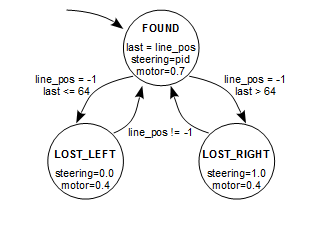
\includegraphics[width=1.0\columnwidth]{images/statemachine} \\
lost track state machine \\
graphical notation
\end{figure}
\end{columns}
\end{frame}


\begin{frame}[fragile]
\frametitle{With State Machines}
Let's make things clearer by following the state machine model: \\
\hfill \\
\begin{columns}[t]
\column{0.646\textwidth}
Write the state actions
\begin{lstlisting}[language=C++,basicstyle=\ttfamily\tiny]
enum State { FOUND, LOST_LEFT, LOST_RIGHT };

void state_action(State state, int16_t line_pos, int16_t& last_out) {
  if (state == FOUND) {
    servo.write((float)line_pos/CAMERA_LENGTH);
    motor = 0.7;
    last = line_pos;
  } else if (state == LOST_LEFT) {
    servo.write(0.0);
    motor = 0.4;
  } else if (state == LOST_RIGHT) {
    servo.write(1.0);
    motor = 0.4;
  }
}
\end{lstlisting}

\column{0.323\textwidth}
\begin{figure}[h!]
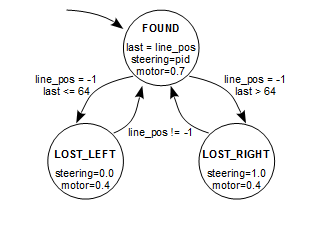
\includegraphics[width=1.0\columnwidth]{images/statemachine} \\
lost track state machine \\
graphical notation
\end{figure}
\end{columns}
\end{frame}


\begin{frame}[fragile]
\frametitle{With State Machines}
Let's make things clearer by following the state machine model: \\
\hfill \\
\begin{columns}[t]
\column{0.646\textwidth}
... and put it all together
\begin{lstlisting}[language=C++,basicstyle=\ttfamily\tiny]
int16_t last = 0;
State state = FOUND;
while (1) {
  int16_t line_pos = line_detect(camera_data);
  state = do_transition(state, line_pos, last);
  state_action(state, line_pos, last);
}
\end{lstlisting}

\column{0.323\textwidth}
\begin{figure}[h!]
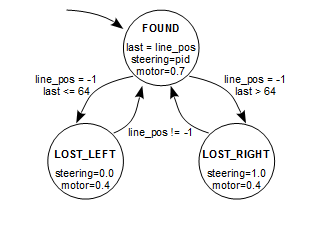
\includegraphics[width=1.0\columnwidth]{images/statemachine} \\
lost track state machine \\
graphical notation
\end{figure}
\end{columns}
\end{frame}


\subsection{Safety-critical code}
%---------------------------------------------------------------------
\begin{frame}[fragile]
\frametitle{Power of Ten}
TODO: power of ten safety critical code guidelines
\end{frame}


\subsection{Other considerations}
%---------------------------------------------------------------------
\begin{frame}[fragile]
\frametitle{Security and Privacy}
So Internet of Things is really hot right now ...
\visible<2-> {
some might even say, \\
\hfill \\
{\centering \textit{it's on fire} \\
\hfill \\
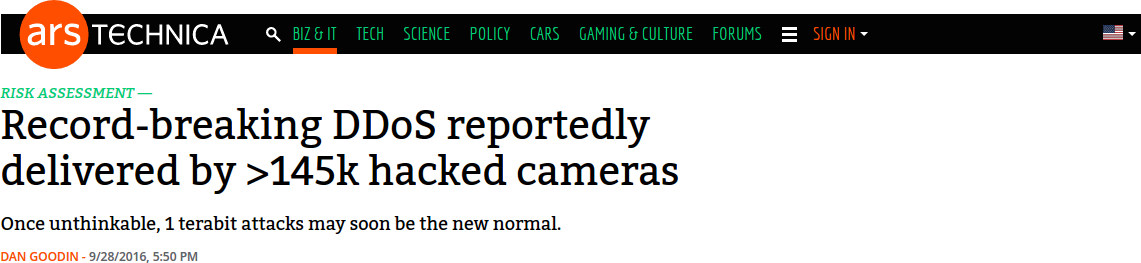
\includegraphics[width=0.7\columnwidth]{external/hacked-headline} \\
\hfill \\
}
What additional concerns are there with Internet-connected devices?
}

\visible<3-> {
\begin{itemize}
  \item Hacking, to become part of a botnet or for data exfiltration
  \begin{itemize}
    \item Common exploits: outdated firmware, default passwords,backdoors, ...
  \end{itemize}
  \item Privacy leaks of user / sensitive data
  \begin{itemize}
    \item Is data encrypted in transit? Is robust authorization in place?
  \end{itemize}
\end{itemize}
}
\end{frame}


%---------------------------------------------------------------------
\section{Summary} % [?? mins]
%---------------------------------------------------------------------

\begin{frame}
\frametitle{Summary}
\begin{itemize}
  \item Optimizations exist if your application is timing sensitive
  \begin{itemize}
    \item Know what to optimize to: no more, no less
    \item I/O probably is the most time consuming operation
  \end{itemize}
  \item Write good code now so you don't kick yourself later
  \begin{itemize}
    \item Understand what your code is doing
    \item Write clear, concise, readable code
    \item Guidelines may be helpful for safety-critical applications
  \end{itemize}  
  \item Be cognizant of the full impact of your software and device
  \begin{itemize}
    \item Security
    \item Privacy
  \end{itemize}  
\end{itemize}
\end{frame}

\end{document}
